\subsection{Field example}
In the next example the field data set had been collected over the Cluny prospect in Mt. Isa area, Queensland, Australia by MIM Exploration Pty, Ltd \cite[]{Rutley01}. The data were collected using pole-dipole and dipole-pole array configuration. The length of the profiles reaches 2000 m in East-West direction. A total of 10 profiles of DC and IP data were collected with electrode spacing of 50 m. There is topographic disturbance along the profile ranging from 429 to 505 meters in absolute elevation above the mean sea level. The DC and IP data, collected over profile 13700 are shown in (Figure \ref{fig:realData}). The data sets were examined for bad data values (outliers) and based on this criterion 45 data had to be eliminated from the IP inversion.
%
\begin{figure}
\centering
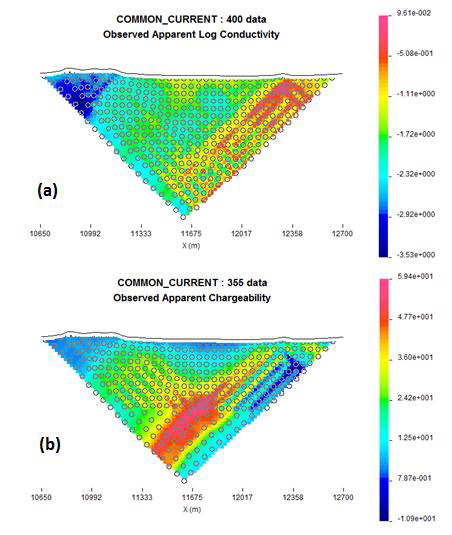
\includegraphics[width=0.5\columnwidth]{realData}
\caption{The observed (a) DC and (b) IP data measured along profile 13700 over the Cluny prospect, Australia.}
\label{fig:realData}
\end{figure}

Resistivity inversion was carried out using the error assignment of 0.0001 base +5\% of the data and constant uniform reference and starting model (100 Ohm m). A default meshing option was used, resulting in 16.8-m wide and 8.33-m high cells in the core region. The control file used for the inversion is provided below with user-defined smallness coefficient and maximum number of iterations set to 50.
%
\begin{fileExample}
\begin{tabular}{|ll|}
\hline
OBS LOC\_X 2D\_13700.dat & ! DC data \\
MESH DEFAULT & ! Created mesh \\
TOPO FILE topo.txt & ! Topography\\
INVMODE SVD & ! Use CG \\
REF\_MOD FILE 1e-2 & ! Reference model \\
INIT\_MOD VALUE 1e-2 & ! Initial model \\
CHIFACT 1 & ! Data misfit to number of data \\
STORE\_ALL\_MODELS TRUE & ! Write out all models \\
ALPHA VALUE 1E-4 1 1 & ! Alpha values \\
NITER 50 & ! Max iterations \\
\hline
\end{tabular}
\end{fileExample}

The results of the inversion (Figure \ref{fig:realDataRec}a) are based on convergence to assigned misfit in 21 iterations (Figure \ref{fig:realDataRec}b). They were compared with the earlier results acquired by \codeName{DCIP3D} code \cite[]{Rutley01} and are shown in Figure \ref{fig:realDataRec}c. The large conductor on the right hand side is a black shale unit. The main geologic structure runs north-south and is essentially perpendicular to the survey line. It is expected therefore that the 2D inversion should produce geologically reasonable results. This is substantiated by comparing this cross-section with a similar cross-section extracted from the 3D inversion (Figures \ref{fig:realDataRec}a and \ref{fig:realDataRec}c).
%
\begin{figure}
\centering
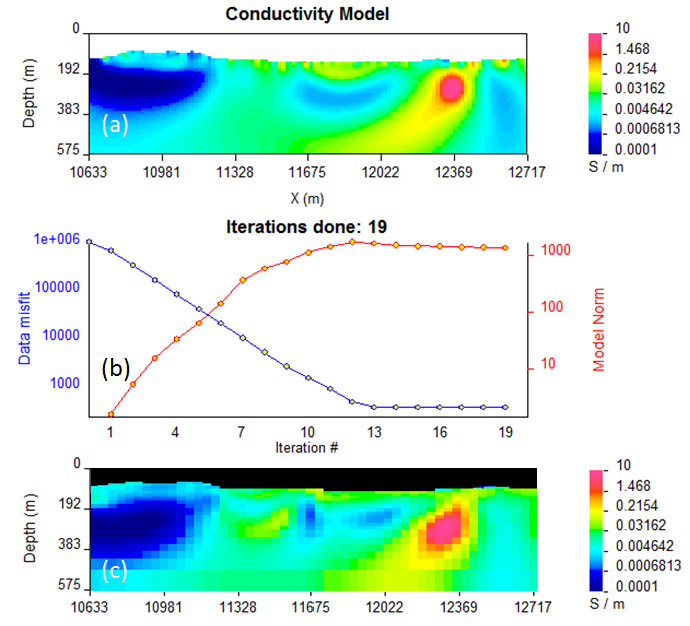
\includegraphics[width=0.5\columnwidth]{realDataRec}
\caption{(a) The recovered model from inverting DC data along profile 13700, Cluny prospect, Queensland, Australia and the associated (b) convergence curves. For reference, (c) the \codeName{DCIP3D} results acquired in 2001 over the same profile.}
\label{fig:realDataRec}
\end{figure}

The conductivity models recovered from the DC inversion were further used to carry out the IP inversion. The IP inversion was carried out using the same mesh as for the DC inversion and was further compared to the 3D inversion carried out previously \cite[]{Rutley01}. Below is the control file used for the IP inversion:
%
\begin{fileExample}
\begin{tabular}{|ll|}
\hline
OBS LOC\_X L13700\_COMPLETE.dat & ! IP data \\
MESH FILE dcinv2d.msh & ! Created mesh from DC inversion\\
TOPO FILE topo.txt & ! Topography\\
INVMODE SVD & ! Use CG \\
REF\_MOD FILE 1e-7 & ! Reference model \\
INIT\_MOD VALUE 1e-7 & ! Initial model \\
CHIFACT 1 & ! Data misfit to number of data \\
STORE\_ALL\_MODELS TRUE & ! Write out all models \\
ALPHA VALUE 1E-4 1 1  & ! Alpha values \\
COND dcinv2d.con & ! Conductivity model \\
NITER 50 & ! Max iterations \\
\hline
\end{tabular}
\end{fileExample}

The results of the inversion were once again compared to the corresponding 3D IP inversion \cite[]{Rutley01} and are shown in Figure ref{fig:realIPres}.
%
\begin{figure}
\centering
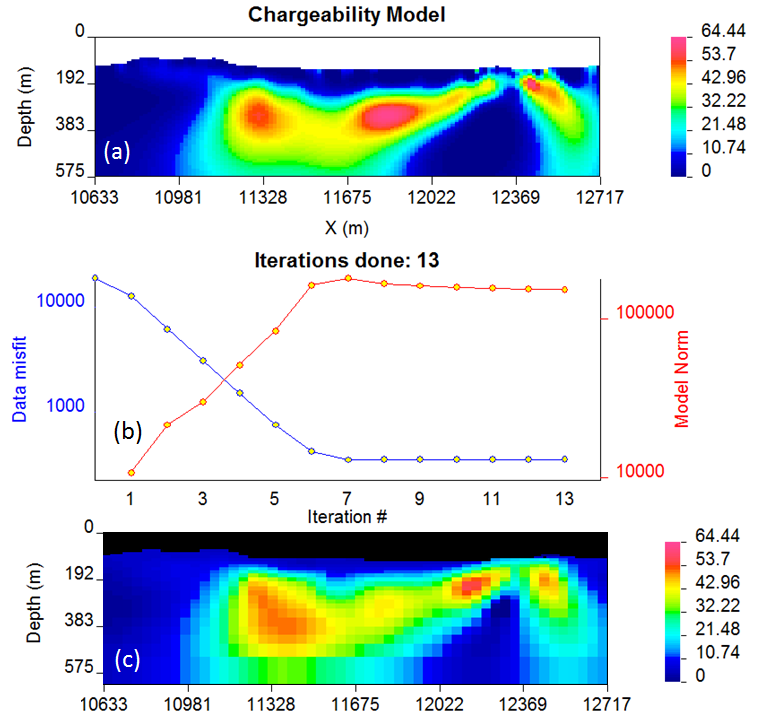
\includegraphics[width=0.5\columnwidth]{realIPres}
\caption{(a) The recovered model from inverting IP data along profile 13700, Cluny prospect, Queensland, Australia and the associated (b) convergence curves. For reference, (c) the \codeName{DCIP3D} results acquired in 2001 over the same profile.}
\label{fig:realIPres}
\end{figure}

The predicted data from the inversions has been verified against the measured data and plotted in Figure \ref{fig:realPre1} and Figure \ref{fig:realPre2}.
%
\begin{figure}
\centering
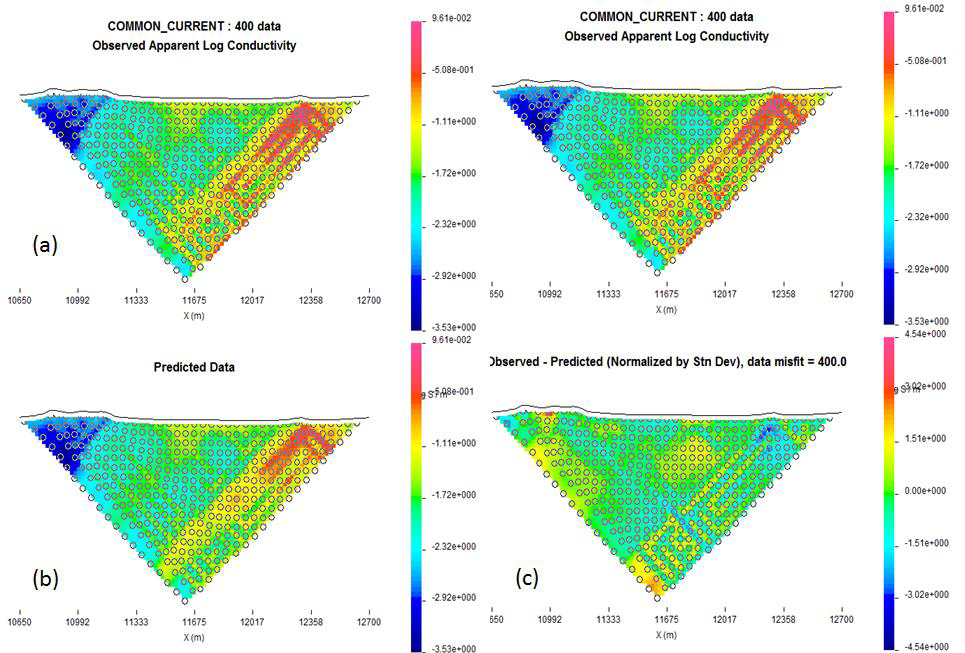
\includegraphics[width=0.5\columnwidth]{realPre1}
\caption{(a) The observed DC data along profile 13700 and (b) the predicted data for comparison. The data misfit normalized by standard deviation is presented in (c).}
\label{fig:realPre1}
\end{figure}
%
\begin{figure}
\centering
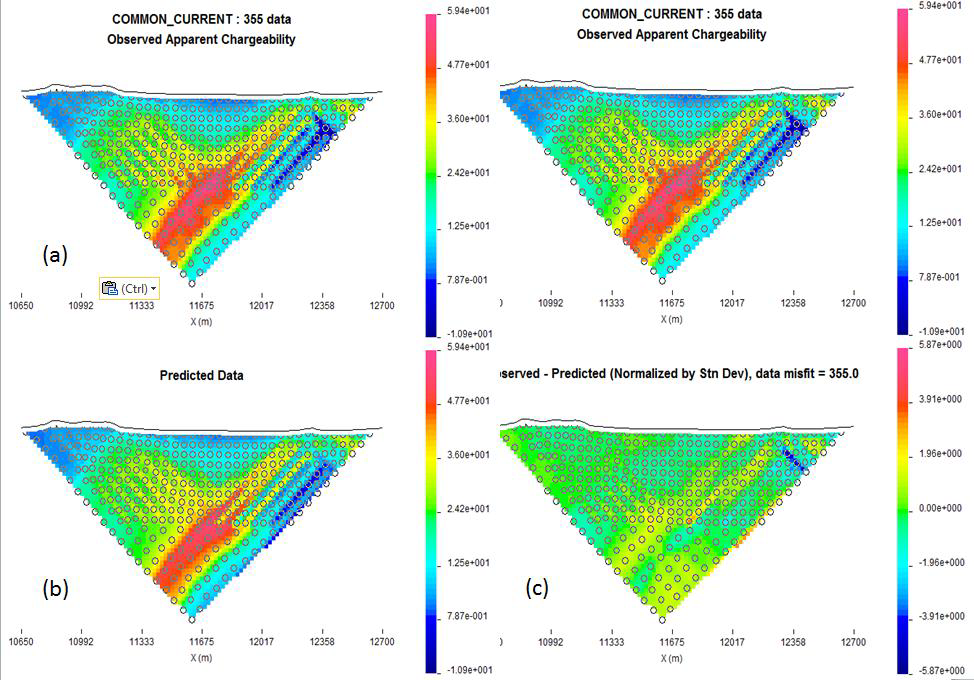
\includegraphics[width=0.5\columnwidth]{realPre2}
\caption{(a) The observed IP data along profile 13700 and (b) the predicted data for comparison. The data misfit normalized by standard deviation is presented in (c).}
\label{fig:realPre2}
\end{figure}
%
Both inversions (DC and IP) have successfully converged and the misfit does not exceed 5 standard deviations, which is one of the criterions of successful inversions. Another criterion is the verification of the 2D results against the 3D results, which show very comparable results.
